%documentclass sets the look of the whole document. you can try changing it around with the two commented out examples.

\documentclass{article}
\usepackage{graphicx}
%\documentclass{proc}
%\documentclass{beamer}


\title{Here is an example of how to use sub-files in LaTeX}

\author{XAM NOSLIW}

\begin{document}
\maketitle

%to include the table of contents just uncoment the line below. The newpage line would move the start of the document on the next page after the table of contents.
%\tableofcontents
%\newpage

\section{Shared Part}

This could be the Shared Part of the document. It is designed to be written by all members of the team.

Each member should ideally write their details in the table of contributors in the Shared Part of the document.

\subsection{Comments from the first student}
The lectures were presented well although short. I like the fact that lots of extra reading resources is available via Moodle.

\subsection{Comments from the second student}
This is the first subsection. Do not forget to include the best parts about the module as well as what you did not like about Max Wilson during the term.

\subsection{Comments from the third student}
This is the first subsection. Do not forget to include the best parts about the module as well as what you did not like about Max Wilson during the term.

\subsection{Comments from the forth student}
This is the first subsection. Do not forget to include the best parts about the module as well as what you did not like about Max Wilson during the term.

\subsection{Comments from the fifth student}
This is the first subsection. Do not forget to include the best parts about the module as well as what you did not like about Max Wilson during the term.

\subsection{Table of Contributors}


If you want to move a table around you will need to put some parameters in square brackets, if you want it exactly where it is positioned in the text editor just uncomment the [h] below, just after begin{table}

This is the table of contributors (Table~\ref{authors}):
\begin{table}%[h]
\centering
\caption{People in the Group}
\label{authors}
\begin{tabular}{|l|l|}
\hline
\textbf{Name} & \textbf{ID} \\
\hline
Aidan Reed & PSYAR8 \\
\hline
Justin Ng & PSYJJN \\
\hline
& \\
\hline
& \\
\hline
& \\
\hline
\end{tabular}
\end{table}
\newpage
\section{First Member}
This is the section dedicated to one of the team members, and it should be written individually . It can include a range of things; first subsection is a space for you to point out the strengths and weaknesses of the module, including complaints about the module coordinator Max Wilson. The second section should have a selfie image with Max! The last part of it is the most important one. You will need to write a paragraph about what you have learned in this module. You can write it in \textbf{Bold} if you want or you can use other fonts. 

Please do not forget:
\begin{itemize}
	\item First paragraph should have your comments about the module
	\item Second one, a selfie img with Max
	\item Last one, what you learned in this module.
\end{itemize}

\subsection{Comments about the module}
The module is well put together in terms of the availability of content (slides, recordings, overview) but I don't feel lectures are utilised effectively as they are often short at around \textbf{35 minutes} per lecture. I also feel that we should have learnt more ways to collaborate  earlier in the module to assist in the accessed labs.

\subsection{Selfie with Max}

\begin{figure}[h]
	\caption{Selfie with Max}
	\centering
	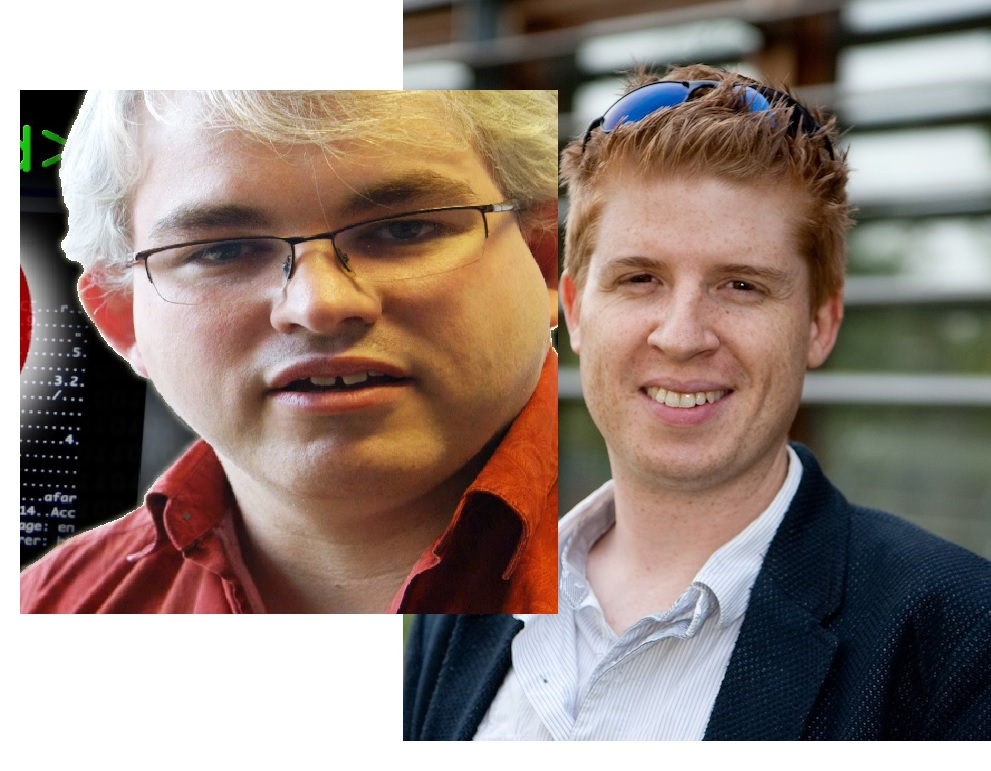
\includegraphics[width=0.5\textwidth]{selfieWithMax}
	\label{fig:selfie}
\end{figure}

My selfie with Max is in  Figure~\ref{fig:selfie}.

\subsection{What I have learned in this module}
I have learnt the importance of working in a team and that communication is key to be able to successfully complete the lab assignments. 


\newpage
\section{Second Member}
This is the section dedicated to one of the team members, and it should be written individually . It can include a range of things; first subsection is a space for you to point out the strengths and weaknesses of the module, including complaints about the module coordinator Max Wilson. The second section should have a selfie image with Max! The last part of it is the most important one. You will need to write a paragraph about what you have learned in this module. You can write it in \textbf{Bold} if you want or you can use other fonts. 

Please do not forget:
\begin{itemize}
	\item First paragraph should have your comments about the module
	\item Second one, a selfie img with Max
	\item Last one, what you learned in this module.
\end{itemize}

\subsection{Comments about the module}
This module has been a different take on what we've seen so far in Computer Science. It's shown us a different take on real life applications of creating software for clients and has highlighted how working in a team is imperative to large or even small scale software creation, driving many people out of their comfort zones and forcing them to adapt to new types of tasks aside from simply coding.

\subsection{Selfie with Max}

To include an image, you will need to remove the comments from the code below, place an image in the main fo lder, and do not forget to put the name of the image instead of ImgName. 

\begin{figure}[h]
	\caption{Selfie with Max}
	\centering
	
\includegraphics[width=0.5\textwidth]{maxnme}
	\label{fig:selfie}
\end{figure}

You can then use the label of the figure to reference it later with the command ${\backslash}ref.$ you can comment out the next line to see an example of how it works.

 My selfie with Max is in  Figure~\ref{fig:selfie}.

\subsection{What I have learned in this module}
I have learned new skills involved less in coding, but more in the surrounding areas of creating software, such as determining clients needs and meeting their expectations. I have also learned how to use new programs such as Visual Paradigm to create models and diagrams with UML. I now understand that making software isn't necessarily about just coding but involves many stages that makes making software a lengthy and deeply constructed process. Another aspect learned is working with other people (of whom I have never met before) which will be an important aspect of creating any software.

\newpage
\section{Third Member}
This is the section dedicated to one of the team members, and it should be written individually . It can include a range of things; first subsection is a space for you to point out the strengths and weaknesses of the module, including complaints about the module coordinator Max Wilson. The second section should have a selfie image with Max! The last part of it is the most important one. You will need to write a paragraph about what you have learned in this module. You can write it in \textbf{Bold} if you want or you can use other fonts. 

Please do not forget:
\begin{itemize}
	\item First paragraph should have your comments about the module
	\item Second one, a selfie img with Max
	\item Last one, what you learned in this module.
\end{itemize}

\subsection{Comments about the module}
The best parts of this module included working in a team which I found challenging yet fun at times.  I found that the lecture was well organised and well structured, however I found that the labs were stressful at times due to having such a limited period of time to complete the work in. 

\subsection{Selfie with Max}
\begin{figure}[h]
\caption{Selfie with Max}
\centering

\includegraphics[width=0.5\textwidth]{imgWithMaxThird}
\label{fig:selfie}
\end{figure}

My selfie with Max is in Figure~\ref{fig:selfie}.

\subsection{What I have learned in this module}
In this module, I have learnt about the development cycle of software, along with agile development and the various testing and objective-gathering methods used in the process.


\newpage
\section{Fourth Member}

\subsection{Comments about the module}
The best part of Software Engineering, was arguably also the worst part, the lab sessions. Working in a team was fun, but could also get stressful due to the looming time constraint. Lectures were dull in all honesty, but I appreciate and realise what is required in the software engineering process, despite how depressing and long winded each of the processes may be. I'm glad we've not had to produce an IEEE SRS Document (yet?). Those standards... intimidate me. 

\subsection{Selfie with Max}

\begin{figure}[h]
\caption{Selfie with Max}
\centering
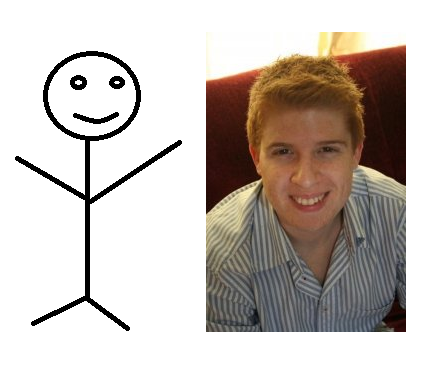
\includegraphics[width=0.5\textwidth]{superiorSelfieWithMax}
\label{fig:selfie}
\end{figure}

\subsection{What I have learned in this module}

In this module I have learnt how to engineer software. 
I have expanded my artistic skills by producing high class (literally!) diagrams.
Have you seen DAT 'SELFIE' btw? BEC DAT SELFIE. (see Figure 4 in Section 5.2)


On a serious note, the most significant aspect within this module has been working towards a deadline in a team. Due to the element of time, we realised there was a requirement for having a strategic approach towards the tasks. Not only did we have to ration out tasks during each lab session, but we would also have regular group meetings in advance during the week, to prepare and ensure we were all on the same level. This is where communication is also very important. In order to maintain consistency we would work together on single word document using Office 365, which I thought was rather useful.


Aside from all that, all the diagrams jazz, etc, etc. You know what I'm on about.

Also screw Visual Paradigm. And Office 365. And tables/images appearing in random places in all of our submitted documents.
\newpage
\section{Fifth Member}
This is the section dedicated to one of the team members, and it should be written individually . It can include a range of things; first subsection is a space for you to point out the strengths and weaknesses of the module, including complaints about the module coordinator Max Wilson. The second section should have a selfie image with Max! The last part of it is the most important one. You will need to write a paragraph about what you have learned in this module. You can write it in \textbf{Bold} if you want or you can use other fonts. 

Please do not forget:
\begin{itemize}
	\item First paragraph should have your comments about the module
	\item Second one, a selfie img with Max
	\item Last one, what you learned in this module.
\end{itemize}

\subsection{Comments about the module}
Studying software engineering was quite interesting. All the lecture slides were very informative and additional information was available in the extended reading section. Working on the group projects were fun and I learnt a lot through it. The module was well laid out; it was easy to follow through. 
\subsection{Selfie with Max}

To include an image, you will need to remove the comments from the code below, place an image in the main folder, and do not forget to put the name of the image instead of ImgName. 

\begin{figure}[h]
\caption{Max}
\centering

\includegraphics[width=0.5\textwidth]{maxWilson}
\label{fig:selfie}
\end{figure}

You can then use the label of the figure to reference it later with the command ${\backslash}ref$. you can comment out the next line to see an example of how it works.

% My selfie with Max is in  Figure~\ref{fig:selfie}.

\subsection{What I have learned in this module}
In this module, I learnt about the various stages involved in software engineering. First of all, we learnt about Requirements engineering. This involves, how to document the requirements laid by the clients, what the difference between requirements and specifications are etc. We then learnt about prototyping which was very interesting. There are 2 different levels of prototyping; high and low. High is often closer to the finished product and low level prototyping is often created using a paper and pen in the initial stages of prototyping. We then went onto study about testing. Testing is an ongoing process with many stages. Acceptance testing is the final part of the project where  the client agrees that the software works as specified and that the project is over now. Another example of testing is release testing, this is when the project managers decide if it's time to release the project. 





\end{document}